\begin{figure}[H]
	\centering
	\begin{subfigure}[t]{0.45\linewidth}
		\centering
		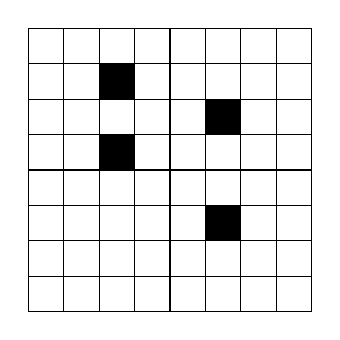
\begin{tikzpicture}[scale=0.45]
			\foreach \x in {(-2, 0), (-2, 2), (1, 1), (1, -2)}
				\filldraw[black] \x rectangle + (1, 1);
			\draw[step=1] (-4, -4) grid (4, 4);
		\end{tikzpicture}
		\caption{Binary image.}
		\label{fig: closingbefore}
	\end{subfigure}
	\hfill
	\begin{subfigure}[t]{0.45\linewidth}
		\centering
		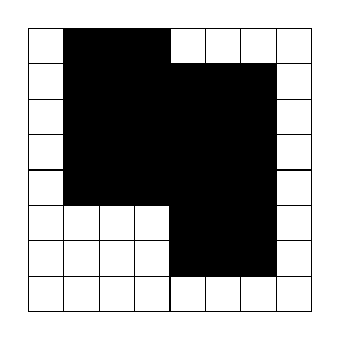
\begin{tikzpicture}[scale=0.45]
			\foreach \x in {(-3, -1), (-3, 0), (-3, 1), (-3, 2), (-3, 3), (-2, -1), (-2, 0), (-2, 1), (-2, 2), (-2, 3), (-1, -1), (-1, 0), (-1, 1), (-1, 2), (-1, 3), (0, -3), (0, -2), (0, -1), (0, 0), (0, 1), (0, 2), (1, -3), (1, -2), (1, -1), (1, 0), (1, 1), (1, 2), (2, -3), (2, -2), (2, -1), (2, 0), (2, 1), (2, 2)}
				\filldraw[black] \x rectangle + (1, 1);
			\draw[step=1] (-4, -4) grid (4, 4);
		\end{tikzpicture}
		\caption{Binary dilation of \ref{fig: closingbefore} with a $3 \times 3$ pixel structuring element.}
		\label{fig: closingdilation}
	\end{subfigure}
	\vfill
	\begin{subfigure}[t]{0.45\linewidth}
		\centering
		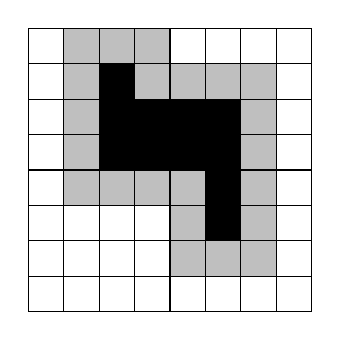
\begin{tikzpicture}[scale=0.45]
			\foreach \x in {(-3, -1), (-3, 0), (-3, 1), (-3, 2), (-3, 3), (-2, -1), (-2, 3), (-1, -1), (-1, 2), (-1, 3), (0, -3), (0, -2), (0, -1), (0, 2), (1, -3), (1, 2), (2, -3), (2, -2), (2, -1), (2, 0), (2, 1), (2, 2)}
				\filldraw[gray, opacity=0.5] \x rectangle + (1, 1);
			\foreach \x in {(-2, 0), (-2, 1), (-2, 2), (-1, 0), (-1, 1), (0, 0), (0, 1), (1, -2), (1, -1), (1, 0), (1, 1)}
				\filldraw[black] \x rectangle + (1, 1);
			\draw[step=1] (-4, -4) grid (4, 4);
		\end{tikzpicture}
		\caption{Result of binary erosion of \ref{fig: closingdilation} with a $3 \times 3$ pixel structuring element. The light gray pixels are set to zero again.}
		\label{fig: closingerosion}
	\end{subfigure}
	\hfill
	\begin{subfigure}[t]{0.45\linewidth}
		\centering
		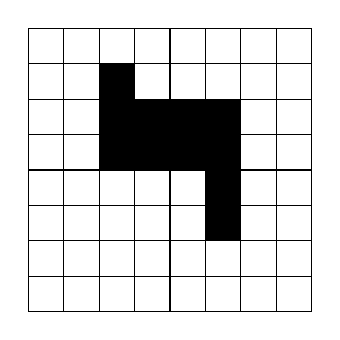
\begin{tikzpicture}[scale=0.45]
			\foreach \x in {(-2, 0), (-2, 1), (-2, 2), (-1, 0), (-1, 1), (0, 0), (0, 1), (1, -2), (1, -1), (1, 0), (1, 1)}
				\filldraw[black] \x rectangle + (1, 1);
			\draw[step=1] (-4, -4) grid (4, 4);
		\end{tikzpicture}
		\caption{Result of closing of \ref{fig: closingbefore} with a $3 \times 3$ pixel structuring element. The gaps between pixels have been filled.}
		\label{fig: closingafter}
	\end{subfigure}
	\caption{Example of binary morphological closing using a $3 \times 3$ pixel structuring element.}
	\label{fig: exampleclosing}
\end{figure}